\section{Evaluation}\label{sec:evaluation}

In this section, we present several applications of imputing objective functions. Furthermore, we first use mathematical modelling to get a convex optimization problem, then we design or apply our approaches and algorithms before implementation. With processing of experimental data and diagrams, we lead a discussion on the performance as well as future work.

\subsection{Curve Fitting}

Curve fitting (\haoyuan{ref}) has widespread applications in data processing among various areas, including big data, machine learning, simulation, noise reduction and so on (\haoyuan{ref}). Interpolation is known as an effective approach for curve fitting. However in this model, we mainly concentrate on a situation of implicit curve fitting. That is to say, we derive an approximate form of the original function by observing the extreme-value points.

We start from a simple example. Suppose the primal function is $f(x)=ax^2+bx$. The values $a$ and $b$ cannot be observed, and hence can only be derived from a set of sample points. As we discussed in the last section, the objective function can be any multiple of $f(x)$. To ensure a unique solution, we model this problem as below.
\begin{align}
\begin{split}\label{quad}
\textrm{minimize }\hspace{.2in}&px+f(x)\\
\textrm{subject to:}\hspace{.2in}&x\ge0
\end{split}
\end{align}

Note that we require $a>0$ so that~(\ref{quad}) is a parameterized convex optimization problem, and we only care about nonnegative solutions. The residues of KKT conditions are
\begin{align*}
r_1 &= -\lambda x\\
r_2 &= p+\nabla f(x)-\lambda
\end{align*}

By~(\ref{p3}), suppose a list of $S$ sample points $(x^*,p)$ are observed from the primal problem~(\ref{quad}). If we assume another quadratic function $\tilde{f}(x)=mx^2+nx$ to fit $f(x)$, we derive the values of $m,n$ by
\begin{align*}
\begin{split}
\textrm{minimize }\hspace{.2in}&\sum_{s=1}^S\left[(2mx_s^*+n+p_s-\lambda_s)^2+(-\lambda_s x_s^*)^2\right]\\
\textrm{subject to:}\hspace{.2in}&\lambda_s\ge0,\hspace{.1in}s=1,\cdots,S
\end{split}
\end{align*}

Another approach for this problem: since $px+\tilde{f}(x)$ reaches the extreme value at $x=-\frac{n+p}{2m}$, we can easily figure out $m,n$ with those sample points by interpolation. But we are not to implement this approach, as we focus more on the performance of the parameterized programming.

\begin{figure}\label{fig:case1}
\centering
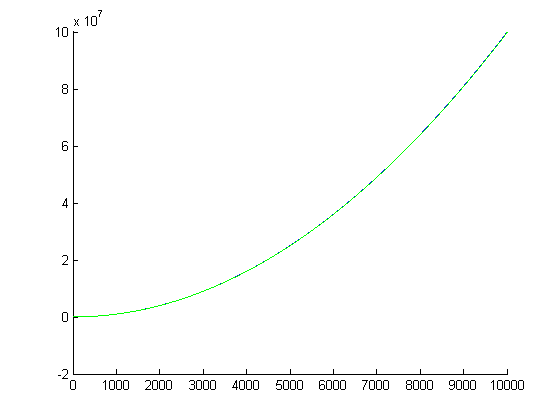
\includegraphics[width=3in]{plots/p1.png}
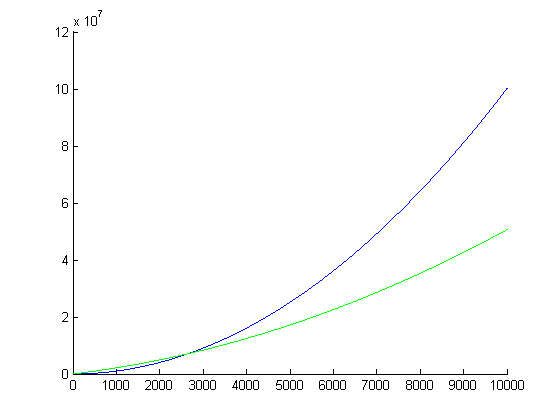
\includegraphics[width=3in]{plots/p2.png}
\caption{Curve fitting. (1) a = 1, b = -10; (2) a = 1, b = 10.}
\end{figure}

Next we conducted the experiment using Matlab 2014a. We randomly select $a=1$, $b=-10$ for the primal problem. 100 sample points are acquired by setting $p\in[2,8]$ with a uniform distribution and solving the primal problem. We draw the curves of the original function and the imputed one together. Figure 1 shows the result, as well as when $a=1$, $b=10$. But the second result has bad performance, because the extreme points are not well covered by sample points.

Some more complicated examples, like the \textit{Consumer Behavior} proposed by~\cite{keshavarz2011}, tends to have further practical use, where a utility function over products is estimated. At that point,

\subsection{Decision Making in Game Theory}

Decision making is an essential concept in game theory, especially the games where players take alternative moves. When designing algorithms for AI in some games to make decisions, the MiniMax algorithm is widely used and considered very effective (\haoyuan{ref}). Usually, given a current state of a 2-player game, to make a decision for the next step, AI will firstly construct a decision tree (say, of depth 10 or so) containing all possible states in next few steps. Then with a pre-prepared evaluation function, it chooses the next move with higher scores and less loss. At that point, the selection of the evaluation function is rather important: the program can only ``look ahead'' a certain number of steps when time is limited. If the evaluation has bad time complexity, the program will be forced to analyze fewer steps, and therefore the performance turns out to be affected. On the other hand, a trivial evaluation function doesn't help much in differentiating various states.

But now we find the approach used for inverse optimization problem is also applicable here. Let's take Gobang as the example, where two players place pieces alternatively. Just like~(\ref{p2}), the parameter $p$ stands for a current state, with some pieces already on the chess board. A solution of the primal problem $x$ just implies the next move, namely where the next piece is placed. Note that given a value $p$, the ``optimal'' solution $x^*$ is usually observed from a big database, or some competitive AI programs (which means our results may fit those programs and be consistent with them). We also build up a space with basic evaluation functions, for example, checking the density of pieces distributed on the board, or how many situations where three pieces are in a row, and so on.

With the approach demonstrated before, we are able to get a combination of those basic functions into a more powerful one, and it can be more practically applicable. But notice that this problem is a different one, in the sense that it's a integer programming problem, so constraints relaxation is necessary somewhere. Unfortunately we didn't get satisfactory results at this point, but it is believed that we can try to improve the model and strive for better performance in future work. 